Computer vision is the computational science aiming at reproducing and improving
the ability of human vision to understand its environment from light sensors.
Throughout a somewhat unconventional, multidisciplinary journey,
this document aims at answering the following question.
How can we leverage user interactions and the Web platform to improve
fields of computer vision such as image segmentation and visual odometry.

On the one hand, image segmentation is the task of identifying precise regions
in an image that are structurally or semantically different.
For medical images, it could be localizing cancer cells while
for urban images, differenciating people, vehicles and traffic signs.
On the other hand, visual odometry consists in analyzing the video stream of a sensor
such as a camera to locate and track its trajectory with regard to its environment.
\alert{Put images illustrating image segmentation and visual odometry?}

Thanks to improvements in imaging and algorithms,
we are now able to automate tasks that were considered science-fiction until recently.
% Let's take self-driving cars as an example.
For instance, some companies~\cite{audia8} claim to have reached level 3
of SAE classification~\cite{sae-cars},
meaning that self-driving vehicle provides autonomy at limited speed,
conditionned by locality and weather among other restrictions.
Nethertheless, we are still far from reaching level 5 of SAE classification
which requires full autonomy in any driving condition.
One non-technical reason is that owners of autonomous vehicles would be reluctant
to accept liability for potential accidents like the incident
of March 18, 2018, that killed Elaine Herzberg~\cite{elaineherzberg}.
I believe that such vehicles will only widespread when they are
safe enough for manufacturers to bear responsability of accidents.
Those capabilities depend on many research fields
including object detection and segmentation of urban images,
as well as visual odometry.
The former is required to detect the road, understand traffic signs,
avoid people, while the latter is needed to precisely record
the vehicle trajectory, especially in situations where other sensors
are not available or sufficiently precise, such as GPS in covered areas.

There exist many approaches for object detection and image segmentation.
Today, the ones performing best rely on a field of research named machine learning.
It consists in building prediction models by aggregating knowledge
from databases of pairs of inputs and outputs called learning datasets.
There are subtleties within the field
and not all algorithms perform equal but the general rule is that
the bigger and most accurate the learning dataset is,
the best will be the detection and segmentation results.
I will thus not focus on machine learning algorithms
but rather on the creation of those datasets.
That process is known as image annotation.
Annotating an image may take different forms depending on the task,
whether it is classification, object detection or segmentation.
In general, it consists in people using image manipulation tools
to draw rectangles, lines, polygons, and other geometric shapes
to identify regions of an image and assign it a label.
The Microsoft COCO dataset~\cite{lin2014microsoft} for example
contains 2.5 million labeled instances accross 328k images annotated by humans,
and required over 22 hours per thousand segmentations.
For a French worker, 35h a week, 228 day a year, this represents approximately 35 years,
almost a full career devoted to that single task.
It is thus understandable that building such datasets must be carefully thought of.

In the first part of this document I will focus on image annotation and segmentation.
Chapter~\ref{cha:the_image_annotation_problem} introduces in more details
the image annotation problem and challenges it brings for large, crowdsourced datasets.
In Chapter~\ref{cha:contribution_outlining}, we focus on the interactive segmentation task.
Many interactions have been explored in the literature to help segmentation algorithms.
The most common consist in designating contours~\cite{russell2008labelme},
bounding boxes around objects~\cite{rother_grabcut:_2004},
or interior and exterior scribbles~\cite{mcguinness2010comparative}.
Crowdsourcing such tasks however implies that non-expert users will have to perform
those interactions and the distinction between expert and non-expert users is rarely touched.
Inspired by the work of Korinke et al.~\cite{korinke_intuitive_2015, korinke_exploring_2015},
we present a user study showing the advantages of the outlining interaction
for crowdsourcing annotations to a non-expert public.
This work has been published at ACM Multimedia 2017~\cite{pizenberg2017outlining}.
Another challenge of crowdsourcing is the distribution medium.
While evaluating an interaction in a small user study does not require complex setup,
distributing an annotation campaign to thousands of potential users might differ.
The best way to proceed is to build a Web application;
and since online annotators are paid for the task,
we need the Web application to be as reliable as possible.
Therefore, in Chapter~\ref{cha:reliable_web_applications} we review evolutions of the Web
since its creation in 1991, especially regarding the development
of reliable frontend applications.
In particular, we describe how the Elm programming language can help us
build a bug-free annotation Web application.
Finally in Chapter~\ref{cha:interactive_annotation_on_the_web},
we present the open source Web application we built for the image annotation task.
A highlights tour of the functionalities and the application architecture is provided,
as well as a guide on how to deploy it to crowdsourcing services
such as Amazon Mechanical Turk.
The presentation of this application was published in the open source competition track
of ACM Multimedia 2018~\cite{pizenberg2018annotation}.


Being a computational science, progress in visual odometry tends to bring larger,
more complex and computationally intensive algorithms over time.
Although beeing a poor unit of measure, number of lines of code provide
an approximation of the relative algorithmic complexity of similar projects.
Let's examine SLAM, which is an extension to visual odometry.
Figure~\ref{fig:assets/img/slam-cloc} illustrates the growth of open source SLAM libraries.
As visible in that figure, projects code bases are growing to unreasonable sizes for research purposes.
This observation is even worse when considering complete structure from motion
libraries such as OpenMVG, reaching 461k lines of code.

\begin{figure}[h]
	\centering
	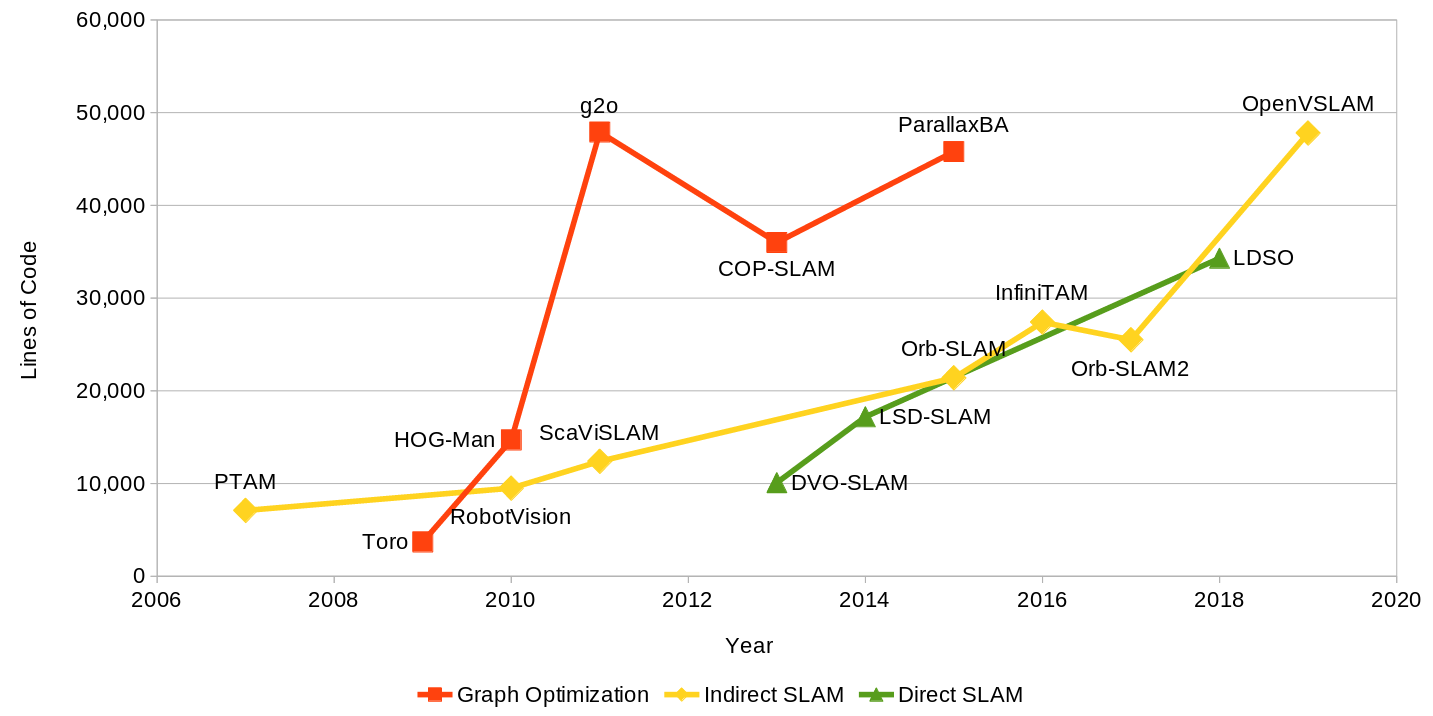
\includegraphics[width=\linewidth]{assets/img/slam-cloc.png}
	\caption{Growth of SLAM libraries over time.}%
	\label{fig:assets/img/slam-cloc}
\end{figure}

Most of SLAM projects are developed using the C++ programming language for performance reasons.
I will argue however, that by continuing to do so, we are hindering mid and long-term research
in the field.
C++ projects are difficult to build, mainly because of assumptions on requirements,
dependency conflicts and usage of Linux, Mac, Windows or architecture specific libraries.
To mitigate those issues, projects tend to include within the source code all of their dependencies.
From the 461k lines of code in OpenMVG, 390k are coming from the \verb|src/nonFree/|
and \verb|src/third_party/| directories.
Although seemingly matters of engineering, those characteristics actually influence research
by putting a very high barrier to entry for new approaches to be able
to reproduce already available results and compare with them.
One should also note that frozing dependency versions is very risky for security concerns,
especially in the context of open source contributions.
\alert{Every contributor should be more careful that the entire Microsoft security team
to avoid 70\% of the CVE related to memory safety in C++}~\cite{msrc-safer}.
Research code will eventually reach critical software, such as autonomous vehicles.
With great research comes great responsability!

\alert{Put more details on contributions here, like for the first part.}
In the second part of this document, we will introduce a new visual odometry library,
started from scratch in the Rust programming language.
It features for example a new points selection algorithm for the camera tracking.
We will also discuss how it has been ported to the Web thanks to a new standard called WebAssembly.
Finally, we will show how we added interactions to the Web application
to improve the tracking and 3D geometry of the visual odometry thanks to user input.
